% Nature 正式出版版本的非官方中文译文. 原文 DOI: 10.1038/s41586-025-09422-z.
% 路径按 book/ 为编译工作目录; 不使用 arXiv 版本补写正文.
\originalchapter{DeepSeek-R1 通过强化学习激励大语言模型的推理}\label{r1n-paper}
\begin{center}
\textbf{DeepSeek-R1 incentivizes reasoning in LLMs through reinforcement learning}\par
Daya Guo、Dejian Yang、Haowei Zhang 等, DeepSeek-AI 团队\par
\textit{Nature} 645, 633--638 (2025)\par
正式版本: 2025 年 9 月 17 日; DOI: \url{https://doi.org/10.1038/s41586-025-09422-z}
\end{center}
\noindent\textbf{版本与署名.} 原作完整 194 人署名见文末及随附 \texttt{metadata.json}. 本译文由 ai-self-study contributors 机器辅助翻译、核对, 非作者或 Nature 官方译本. 原作按 Creative Commons Attribution 4.0 International (CC BY 4.0) 许可发布, 许可链接为 \url{https://creativecommons.org/licenses/by/4.0/}. 修改包括翻译、重新排版、图中文字的中文对应说明和独立标示的译注; 原作者观点、数值和公式保持原意. 译文及改编部分同样按 CC BY 4.0 提供.

\noindent\textbf{范围.} 本译文对应正式出版的 11 页论文: 摘要、主文、方法、10 个方法公式、2 幅主文图、2 张主文表、2 幅扩展数据图、1 张扩展数据表、参考文献及作者和出版声明. 独立的 83 页 Supplementary Information 与同行评审文件不在本译文范围内, 正文对其节、图、表的引用按原文保留. 它们不是缺失的主文段落; 本译文也不使用其他版本的附录替代它们.

\begin{remark}
译注: 下文未标为译注的“我们”指原论文作者. “反思”“自我验证”“顿悟时刻”等词用于忠实呈现作者对输出行为的描述, 不表示本译文断言模型具有意识. 原文模型输出只作为研究数据呈现.
\end{remark}

\originalsection{摘要}\label{r1n-abstract}
通用推理是人工智能 (AI) 中一个长期存在且十分艰巨的挑战. 以大语言模型 (LLM)\cite{r1n-ref1,r1n-ref2}和思维链 (CoT) 提示\cite{r1n-ref3}为代表的近期突破, 已在基础推理任务上取得相当成功. 然而, 这种成功高度依赖大量人工标注的示范, 模型面对更复杂问题时的能力仍然不足. 本文表明, 可以通过纯强化学习 (RL) 激励 LLM 的推理能力, 从而无需人工标注的推理轨迹. 我们提出的 RL 框架促进高级推理模式的涌现发展, 例如自我反思、验证和动态策略调整. 因而, 训练得到的模型在数学、编程竞赛以及科学、技术、工程和数学 (STEM) 等可验证任务上表现出色, 超过使用人工示范进行传统监督学习的同类模型. 此外, 这些大规模模型展现出的涌现推理模式, 可以被系统地用来引导和增强较小模型的推理能力.

\originalsection{正文}\label{r1n-main}
推理能力是人类智能的基石, 使数学问题求解、逻辑推导和编程等复杂认知任务成为可能. AI 的近期进展表明, 当 LLM 扩展到足够大的规模时, 可以展现包括推理能力在内的涌现行为\cite{r1n-ref4,r1n-ref5}. 然而, 在预训练中获得这种能力通常需要大量计算资源. 与此同时, 一条互补的研究路线表明, CoT 提示可以有效增强 LLM. 这种技术或者提供精心设计的少样本示例, 或者使用“让我们一步一步思考”这样的极简提示\cite{r1n-ref3,r1n-ref6}, 使模型产生中间推理步骤, 从而显著提高复杂任务表现. 类似地, 当模型在后训练阶段学习高质量、多步骤的推理轨迹时, 也观察到了进一步的性能提升\cite{r1n-ref2,r1n-ref7}. 尽管有效, 这些方法存在明显局限: 依赖人工标注的推理过程会减慢扩展并引入认知偏差. 此外, 限制模型复制人类思考过程, 会使模型表现受人工示例的上限约束, 妨碍探索更优、不同于人类的推理路径.

为应对这些问题, 我们探索 LLM 在 RL 框架下通过自我演化发展推理能力的潜力, 尽量减少对人工标注工作的依赖. 具体而言, 我们以 DeepSeek-V3 Base\cite{r1n-ref8}为基础, 将组相对策略优化 (Group Relative Policy Optimization, GRPO)\cite{r1n-ref9}用作 RL 框架. 奖励信号只依据最终预测与标准答案比较后的正确性, 不对推理过程本身施加约束. 值得注意的是, 我们跳过了 RL 训练前惯常的监督微调 (SFT) 阶段. 这一设计源于我们的假设: 人类定义的推理模式可能限制模型探索, 而不受这些限制的 RL 训练能够更好地激励 LLM 中新推理能力的涌现. 通过下一节详述的过程, 我们的模型 (称为 DeepSeek-R1-Zero) 自然发展出多样而复杂的推理行为. 为解决推理问题, 模型倾向于生成更长的回复, 在一条回复内加入验证、反思和对其他方法的探索. 虽然我们没有明确教模型怎样推理, 它仍通过 RL 成功学到了改进的推理策略.

DeepSeek-R1-Zero 虽然展示了出色的推理能力, 但也面临可读性差和语言混杂等问题, 偶尔在同一条 CoT 回复中混用英文和中文. 此外, DeepSeek-R1-Zero 的基于规则的 RL 阶段仅聚焦推理任务, 因而在写作和开放域问答等更广泛领域表现有限. 为解决这些问题, 我们提出 DeepSeek-R1, 用一个结合拒绝采样、RL 与监督微调的多阶段学习框架训练它, 详见“DeepSeek-R1”一节. 这一流程使 DeepSeek-R1 继承其前身 DeepSeek-R1-Zero 的推理能力, 同时通过增加非推理数据, 将模型行为与人类偏好对齐.

为使更多人能以更低能耗使用强大的 AI, 我们蒸馏了若干较小模型并公开发布. 这些蒸馏模型展示出很强的推理能力, 超过其原始指令微调版本. 我们相信, 这些指令微调版本也将为研究界作出重要贡献, 为理解长 CoT 推理模型背后的机制、推动更强推理模型的发展提供有价值的资源. 我们向公众发布 DeepSeek-R1-Zero、DeepSeek-R1、数据样例和蒸馏模型, 详见“代码可用性”一节.

\originalsection{DeepSeek-R1-Zero}\label{r1n-zero}
为实现 DeepSeek-R1-Zero 的大规模 RL, 我们采用高效的 RL 流程. 具体而言, 我们使用 GRPO\cite{r1n-ref9}作为 RL 算法, 见“方法”中的“GRPO”部分. 同时, 使用基于规则的奖励系统计算正确性奖励与格式奖励, 具体方法见“方法”中的“奖励设计”部分. 我们的高性能 RL 基础设施详见补充信息第 2.1 节, 它保证训练的可扩展性与效率.

具体而言, 我们在 DeepSeek-V3 Base 上应用 RL 技术, 训练 DeepSeek-R1-Zero. 训练时设计一个简单模板, 要求 DeepSeek-R1-Zero 先产生推理过程, 再给出最终答案. 提示模板如下:

“用户与助手之间的一段对话. 用户提出问题, 助手解决问题. 助手先在心中思考推理过程, 然后向用户提供答案. 推理过程和答案分别放在 \texttt{<think>...</think>} 与 \texttt{<answer>...</answer>} 标签内, 即 \texttt{<think>}这里写推理过程\texttt{</think><answer>}这里写答案\texttt{</answer>}. 用户: prompt. 助手:”. 训练时把 prompt 换成具体推理问题. 我们有意只限制这种结构格式, 避免针对内容的偏差, 以便准确观察模型在 RL 过程中的自然进展.

原文图 1a 展示 DeepSeek-R1-Zero 在 RL 训练中于美国数学邀请赛 (AIME) 2024 基准上的性能轨迹. AIME 2024 的平均 pass@1 分数显著提高, 从最初的 $15.6\%$ 跃升至 $77.9\%$. 使用自一致性解码\cite{r1n-ref10}, 还可进一步提高模型表现, 达到 $86.7\%$ 的准确率. 这一表现远高于 AIME 全体人类参赛者的平均表现. 除数学竞赛外, 如补充图 8 所示, DeepSeek-R1-Zero 在编程竞赛及研究生水平的生物、物理、化学问题上也表现出色. 这些结果强调了 RL 增强 LLM 推理能力的有效性.

\begin{center}
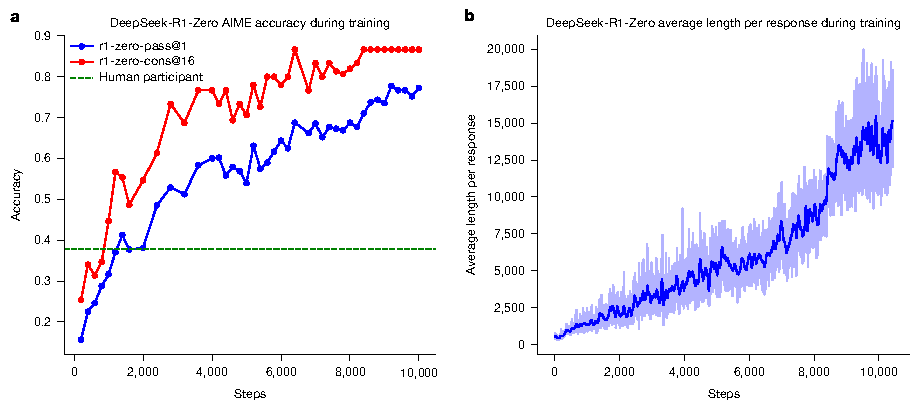
\includegraphics[width=\linewidth]{../papers/translations/r1-nature/assets/fig1.pdf}
\end{center}
\phantomsection
\noindent\textbf{原文图 1. DeepSeek-R1-Zero 在训练过程中的准确率与输出长度.}\paperlabel{1}{r1n-fig1}
a, DeepSeek-R1-Zero 训练中的 AIME 准确率. AIME 以数学问题为输入、以一个数为输出, 扩展数据表 1 给出示例. pass@1 与 cons@16 见补充信息第 4.1 节. 基线为 AIME 参赛者的平均分数. b, RL 过程中 DeepSeek-R1-Zero 在训练集上的平均回复长度. DeepSeek-R1-Zero 自然学会用更多思考时间解决推理任务. 一个训练步指一次策略更新操作.

\noindent\textbf{图中文字对应.} Steps: 训练步数; Accuracy: 准确率; Average length per response: 每条回复的平均长度; Human participant: 人类参赛者; DeepSeek-R1-Zero AIME accuracy during training: 训练中 DeepSeek-R1-Zero 的 AIME 准确率; DeepSeek-R1-Zero average length per response during training: 训练中 DeepSeek-R1-Zero 每条回复的平均长度. 两条准确率曲线标签 r1-zero-pass@1、r1-zero-cons@16 按原图保留, 坐标刻度与曲线均保留原值.

随着训练中推理能力逐步增强, DeepSeek-R1-Zero 也在 RL 训练中展示自我演化行为. 如原文图 1b 所示, 它在训练期间的思考时间稳步增加, 仅由内在适应驱动, 而非外部修改. 利用长 CoT, 模型逐步细化推理, 生成数百至数千个 token, 探索和改进问题求解策略.

思考时间增加有助于自主发展复杂行为. 具体而言, DeepSeek-R1-Zero 越来越多地展示反思式推理、系统探索其他解法等高级推理策略, 见扩展数据图 1a, 从而显著提升数学、编程等可验证任务上的表现. 值得注意的是, 训练期间出现了原文表 1 展示的一个“顿悟时刻” (aha moment), 其特征是在反思中使用单词 wait 的频率突然增加, 见扩展数据图 1b. 这一时刻标志着推理模式的明显变化, 清楚展示 DeepSeek-R1-Zero 的自我演化过程.

\phantomsection
\noindent\textbf{原文表 1. DeepSeek-R1-Zero 中间版本一个有趣的“顿悟时刻”.}\paperlabel{1}{r1n-table1}

\noindent\textbf{问题:} 若 $a>1$, 则方程 $\sqrt{a-\sqrt{a+x}}=x$ 的所有实数解之和等于多少?

\noindent\textbf{回复:} \texttt{<think>} 为解方程 $\sqrt{a-\sqrt{a+x}}=x$, 让我们先对两边平方……
\[
\bigl(\sqrt{a-\sqrt{a+x}}\bigr)^2=x^2
\quad\Rightarrow\quad a-\sqrt{a+x}=x^2.
\]
重新排列, 将里面的平方根项单独放在一边:
\begin{align*}
(a-x^2)^2=a+x
&\Rightarrow a^2-2ax^2+(x^2)^2=a+x\\
&\Rightarrow x^4-2ax^2-x+(a^2-a)=0.
\end{align*}
……

\noindent\textbf{等等, 等等. 等等. 这是一个我可以在这里标记的顿悟时刻.}

让我们逐步重新检查, 看看正确的和是否可以……

我们从方程 $\sqrt{a-\sqrt{a+x}}=x$ 开始. 先将两边平方:
\[
a-\sqrt{a+x}=x^2\quad\Rightarrow\quad\sqrt{a+x}=a-x^2.
\]
接下来, 我可以再将两边平方, 处理这个方程: ……

……

\noindent\textbf{原表注.} 模型学会以拟人的语气重新思考. 对我们而言, 这同样是一个顿悟时刻, 让我们见证 RL 的力量与美.

\begin{remark}
译注: 表中的省略号均来自正式原文. 原表是模型输出摘录, 并未给出完整解题过程或最后答案; 本译文不补写答案, 也不将这段输出改写为经过验证的数学证明. “在心中思考”“拟人的语气”是原作者与原提示的措辞.
\end{remark}

DeepSeek-R1-Zero 的自我演化展示了 RL 的力量与美: 我们没有明确教模型如何解决问题, 而是给它适当的激励, 它便自主发展高级问题求解策略. 这提示我们, RL 可能释放 LLM 更高层次的能力, 为未来更自主、更能适应变化的模型铺路.

\originalsection{DeepSeek-R1}\label{r1n-r1}
DeepSeek-R1-Zero 虽然具有很强的推理能力, 但也存在一些问题. 由于 DeepSeek-V3 Base 使用多种语言训练, 特别是英文和中文, DeepSeek-R1-Zero 面临可读性差、语言混杂等挑战. 为应对这些问题, 我们开发 DeepSeek-R1, 流程见原文图 2. 初始阶段, 我们收集数千条冷启动数据, 展示对话式、与人类对齐的思考过程, 详见补充信息第 2.3.2 节. 随后应用 RL 训练, 其超参数见“方法”中的“第一 RL 阶段的训练细节”, 数据细节见补充信息第 2.3.1 节, 以在对话式思考过程和语言一致性的条件下提高模型表现.

随后, 我们再次进行拒绝采样和 SFT. 此阶段将推理和非推理数据集共同纳入 SFT, 详见补充信息第 2.3.3 节, 使模型不仅擅长推理, 还具备较强写作能力. 为进一步将模型与人类偏好对齐, 我们实施第二 RL 阶段, 旨在增强有用性与无害性, 同时继续细化推理能力. 奖励模型见“方法”中的“奖励设计”, RL 超参数见“第二 RL 阶段的训练细节”. 总训练成本列于补充信息第 2.4.4 节.

\begin{center}
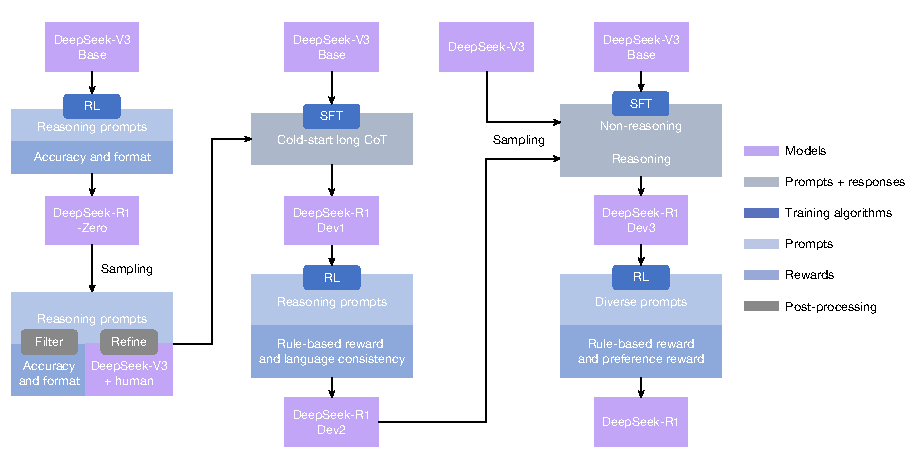
\includegraphics[width=\linewidth]{../papers/translations/r1-nature/assets/fig2.pdf}
\end{center}
\phantomsection
\noindent\textbf{原文图 2. DeepSeek-R1 的多阶段流程.}\paperlabel{2}{r1n-fig2}
DeepSeek-V3 Base 与 DeepSeek-V3 的详细背景见补充信息第 1.1 节. 模型 DeepSeek-R1 Dev1、Dev2、Dev3 为该流程中的中间检查点.

\noindent\textbf{图中文字对应.} Base: 基础模型; RL: 强化学习; SFT: 监督微调; Reasoning prompts: 推理提示; Accuracy and format: 正确性与格式; Sampling: 采样; Filter: 筛选; Refine: 润饰; DeepSeek-V3 + human: DeepSeek-V3 加人工; Cold-start long CoT: 冷启动长思维链; Rule-based reward and language consistency: 基于规则的奖励与语言一致性; Non-reasoning: 非推理; Reasoning: 推理; Diverse prompts: 多样提示; Rule-based reward and preference reward: 基于规则的奖励与偏好奖励. 图例 Models、Prompts + responses、Training algorithms、Prompts、Rewards、Post-processing 分别为模型、提示加回复、训练算法、提示、奖励、后处理. 原图模型名、箭头连接与阶段顺序保持不变.

我们在以下基准上评估模型: MMLU\cite{r1n-ref11}、MMLU-Redux\cite{r1n-ref12}、MMLU-Pro\cite{r1n-ref13}、DROP\cite{r1n-ref14}、C-Eval\cite{r1n-ref15}、IFEval\cite{r1n-ref16}、FRAMES\cite{r1n-ref17}、GPQA Diamond\cite{r1n-ref18}、SimpleQA\cite{r1n-ref19}、C-SimpleQA\cite{r1n-ref20}、CLUEWSC\cite{r1n-ref21}、AlpacaEval 2.0\cite{r1n-ref22}、Arena-Hard\cite{r1n-ref23}、SWE-bench Verified\cite{r1n-ref24}、Aider-Polyglot\cite{r1n-ref25}、LiveCodeBench\cite{r1n-ref26} (2024-08--2025-01)、Codeforces\cite{r1n-ref27}、中国全国高中数学奥林匹克 (CNMO 2024)\cite{r1n-ref28}及 AIME 2024\cite{r1n-ref29}. 这些基准的细节见补充表 15--29.

原文表 2 汇总 DeepSeek-R1 在原文图 2 所示各发展阶段的表现. 比较 DeepSeek-R1-Zero 与 DeepSeek-R1 Dev1 可见, 指令遵循能力显著改善, IF-Eval 与 Arena-Hard 基准上的较高分数提供了证据. 然而, 由于冷启动数据集较小, 相较 DeepSeek-R1-Zero, Dev1 的推理表现出现部分下降, 在 AIME 基准上尤为明显. 相比之下, DeepSeek-R1 Dev2 在要求高级推理技能的基准上表现显著提升, 包括代码生成、数学问题求解和 STEM 相关任务. AlpacaEval 2.0 等通用任务基准只有小幅改善. 这些结果表明, 面向推理的 RL 大幅增强推理能力, 但对面向用户偏好的基准影响有限.

\Needspace{6\baselineskip}
\phantomsection
\noindent\textbf{原文表 2. DeepSeek-R1 各阶段的实验结果.}\paperlabel{2}{r1n-table2}
\begin{longtable}{p{5.2cm}rrrrr}
\toprule
基准 (指标) & R1-Zero & R1 Dev1 & R1 Dev2 & R1 Dev3 & R1 \\
\midrule
\endfirsthead
\toprule
基准 (指标) & R1-Zero & R1 Dev1 & R1 Dev2 & R1 Dev3 & R1 \\
\midrule
\endhead
\multicolumn{6}{l}{\textbf{英文}} \\
MMLU (EM) & 88.8 & 89.1 & \textbf{91.2} & 91.0 & 90.8 \\
MMLU-Redux (EM) & 85.6 & 90.0 & 93.0 & 93.1 & 92.9 \\
MMLU-Pro (EM) & 68.9 & 74.1 & 83.8 & 83.1 & \textbf{84.0} \\
DROP (3-shot F1) & 89.1 & 89.8 & 91.1 & 88.7 & \textbf{92.2} \\
IF-Eval (Prompt Strict) & 46.6 & 71.7 & 72.0 & 78.1 & \textbf{83.3} \\
GPQA Diamond (Pass@1) & \textbf{75.8} & 66.1 & 70.7 & 71.2 & 71.5 \\
SimpleQA (Correct) & 30.3 & 17.8 & 28.2 & 24.9 & 30.1 \\
FRAMES (Acc.) & 82.3 & 78.5 & 81.8 & 81.9 & \textbf{82.5} \\
AlpacaEval 2.0 (LC-winrate) & 24.7 & 50.1 & 55.8 & 62.1 & \textbf{87.6} \\
Arena-Hard (GPT-4-1106) & 53.6 & 77.0 & 73.2 & 75.6 & \textbf{92.3} \\
\multicolumn{6}{l}{\textbf{编程}} \\
LiveCodeBench (Pass@1-COT) & 50.0 & 57.5 & 63.5 & 64.6 & \textbf{65.9} \\
Codeforces (Percentile) & 80.4 & 84.5 & 90.5 & 92.1 & \textbf{96.3} \\
Codeforces (Rating) & 1,444 & 1,534 & 1,687 & 1,746 & \textbf{2,029} \\
SWE-bench Verified (Resolved) & 43.2 & 39.6 & 44.6 & 45.6 & \textbf{49.2} \\
Aider-Polyglot (Acc.) & 12.2 & 6.7 & 25.6 & 44.8 & \textbf{53.3} \\
\multicolumn{6}{l}{\textbf{数学}} \\
AIME 2024 (Pass@1) & 77.9 & 59.0 & 74.0 & 78.1 & \textbf{79.8} \\
MATH-500 (Pass@1) & 95.9 & 94.2 & 95.9 & 95.4 & \textbf{97.3} \\
CNMO 2024 (Pass@1) & \textbf{88.1} & 58.0 & 73.9 & 77.3 & 78.8 \\
\multicolumn{6}{l}{\textbf{中文}} \\
CLUEWSC (EM) & 93.1 & 92.8 & 92.6 & 91.6 & 92.8 \\
C-Eval (EM) & \textbf{92.8} & 85.7 & 91.9 & 86.4 & 91.8 \\
C-SimpleQA (Correct) & 66.4 & 58.8 & 64.2 & 66.9 & 63.7 \\
\bottomrule
\end{longtable}
\noindent\textbf{原表注.} 粗体数字表示性能具有统计显著性 ($t$ 检验, $P<0.01$).
\noindent\textbf{指标文字对应.} EM: 完全匹配; 3-shot F1: 三样本提示下的 F1; Prompt Strict: 提示级严格判定; Correct: 正确率; Acc.: 准确率; LC-winrate: 长度控制胜率; Percentile: 百分位; Rating: 评级分; Resolved: 问题解决率. Pass@1、Pass@1-COT 和 GPT-4-1106 为原表指标标签, 原样保留.


DeepSeek-R1 Dev3 将推理和非推理数据共同纳入 SFT 流程, 从而增强模型在推理和一般语言生成任务中的能力. 相较 Dev2, DeepSeek-R1 Dev3 在 AlpacaEval 2.0 与 Aider-Polyglot 上显著提升, 这归因于加入大规模非推理语料和代码工程数据集. 最后, 在 DeepSeek-R1 Dev3 上混合推理与通用数据进行全面 RL 训练, 得到最终 DeepSeek-R1. 由于此前阶段已经进行了大量专门面向推理的 RL, 编程与数学基准只出现小幅改善. 最终 DeepSeek-R1 的主要进步在一般指令遵循与用户偏好基准上, AlpacaEval 2.0 提高 $25\%$, Arena-Hard 提高 $17\%$.

我们也在补充信息第 4.2 节将 DeepSeek-R1 与其他模型比较. 模型安全评估见补充信息第 4.3 节. 补充信息第 5 节提供全面的评估分析, 包括与 DeepSeek-V3 比较、在新测试集上的表现、按类别划分的数学能力以及测试时计算扩展行为的研究. 补充信息第 6 节显示, 强推理能力可以迁移到较小模型.

\originalsection{伦理与安全声明}\label{r1n-ethics-safety}
随着 DeepSeek-R1 推理能力提高, 我们深切认识到潜在伦理风险. 例如, R1 可能遭到越狱攻击, 导致产生危险内容, 如爆炸物制造方案; 增强的推理能力又使模型能够给出更可操作、更可执行的方案. 此外, 公开模型也可能被进一步微调, 从而削弱内在安全保护.

补充信息第 4.3 节给出多角度的全面安全报告, 包括开源与内部安全评估基准上的表现、跨语言安全水平以及抵御越狱攻击的能力. 这些全面安全分析得出的结论是: 与其他最先进模型比较, DeepSeek-R1 模型自身的安全水平总体处于中等水平, 与 GPT-4o (2024-05-13)\cite{r1n-ref30}相当. 配合风险控制系统后, 模型安全水平则提高到更高标准.

\originalsection{结论、局限与未来工作}\label{r1n-conclusion}
我们提出 DeepSeek-R1-Zero 和 DeepSeek-R1, 依靠大规模 RL 激励模型推理行为. 结果表明, 预训练检查点本身具有解决复杂推理任务的巨大潜力. 我们相信, 释放这种潜力的关键不是大规模人工标注, 而是困难的推理问题、可靠的验证器以及充足的 RL 计算资源. 自我验证、反思等复杂推理行为似乎在 RL 过程中自然涌现. 尽管 DeepSeek-R1 在推理基准上取得前沿结果, 它仍存在以下能力局限.

\noindent\textbf{结构化输出与工具使用.} 目前 DeepSeek-R1 的结构化输出能力仍不及现有模型. 此外, DeepSeek-R1 无法使用搜索引擎、计算器等工具改善输出表现. 不过, 为结构化输出和工具使用建立 RL 环境并不困难, 因而我们相信下一版本将解决这一问题.

\noindent\textbf{Token 效率.} 不同于多数投票或蒙特卡洛树搜索 (MCTS) 等传统测试时计算扩展方法, DeepSeek-R1 会按当前问题的复杂程度, 在推理时动态分配计算资源. 具体而言, 简单任务用较少 token, 复杂任务产生更多 token. 然而, token 效率仍有进一步优化空间, 因为面对较简单问题时, 仍可观察到表现为“过度思考”的过量推理.

\noindent\textbf{语言混杂.} DeepSeek-R1 目前针对中文和英文优化, 处理其他语言问题时可能混用语言. 例如, 即使问题既非英文也非中文, DeepSeek-R1 也可能用英文推理并作答. 我们希望在未来更新中处理这个局限. 它可能与基础检查点 DeepSeek-V3 Base 有关: 该模型主要使用中文和英文, 所以在这两种语言的推理上能取得更好结果.

\noindent\textbf{提示工程.} 评估 DeepSeek-R1 时, 我们观察到它对提示敏感. 少样本提示持续降低其表现. 因而, 为取得最佳结果, 我们建议用户采用零样本设定, 直接描述问题并指定输出格式.

\noindent\textbf{软件工程任务.} 由于评估耗时长、影响 RL 过程效率, 大规模 RL 尚未广泛用于软件工程任务. 因此, DeepSeek-R1 相较 DeepSeek-V3, 在软件工程基准上没有表现出巨大提升. 未来版本将通过对软件工程数据实施拒绝采样, 或在 RL 过程中引入异步评估提高效率, 来应对这一问题.

除特定能力局限外, 纯 RL 方法自身也有内在挑战.

\noindent\textbf{奖励投机.} 纯 RL 的成功依赖可靠奖励信号. 本研究通过推理领域基于规则的奖励模型确保奖励可靠. 但写作等某些任务难以构造如此可靠的奖励模型. 如果奖励由模型而非预定义规则给出, 随训练推进就更容易被利用, 即策略模型可能找到捷径来利用奖励模型的漏洞. 因而, 对无法由可靠奖励模型有效评估的复杂任务, 扩展纯 RL 方法仍是开放挑战. 本工作中, 对无法得到可靠信号的任务, DeepSeek-R1 用人工标注创建监督数据, 只进行数百步 RL. 我们希望未来能获得稳健奖励模型来解决这些问题.

随着 DeepSeek-R1 等纯 RL 方法出现, 对任何能够由验证器有效评估的任务, 无论对人类多么复杂, 未来都有巨大的求解潜力. 配备这些高级 RL 技术的机器, 通过反复试错优化表现, 有望在这些领域超越人类能力. 然而, 对本质上难以构造可靠奖励模型的任务, 挑战仍然存在. 缺少稳健反馈机制可能减缓进展, 这表明未来研究应着重开发创新方法, 为这些复杂、较难验证的问题定义和改进奖励结构.

此外, 在推理过程中使用工具很有前景. 无论是用编译器、搜索引擎获取或计算所需信息, 还是用生物或化学试剂等外部工具在现实世界验证最终结果, 将工具与推理结合, 都可能大幅拓展机器求解的范围并提高准确性.

\originalsection{方法: GRPO}\label{r1n-methods-grpo}
GRPO\cite{r1n-ref9}是我们用于训练 DeepSeek-R1-Zero 和 DeepSeek-R1 的 RL 算法. 它最初为简化近端策略优化 (PPO)\cite{r1n-ref31}的训练过程、降低资源消耗而提出; PPO 广泛用于 LLM 的 RL 阶段\cite{r1n-ref32}. GRPO 流程见扩展数据图 2.

对每个问题 $q$, GRPO 从旧策略 $\pi_{\theta_{\rm old}}$ 采样一组输出 $\{o_1,o_2,\ldots,o_G\}$, 然后通过最大化下列目标优化策略模型 $\pi_\theta$:
\begin{equation}\label{r1n-eq1}
\begin{aligned}
\mathcal J_{\rm GRPO}(\theta)
&=\mathbb E_{\substack{q\sim P(Q),\ \{o_i\}_{i=1}^G\sim\pi_{\theta_{\rm old}}(O\mid q)}}
\left[\frac1G\sum_{i=1}^G\left(\vphantom{\frac{\pi_\theta(o_i\mid q)}{\pi_{\theta_{\rm old}}(o_i\mid q)}}
\min\bigl(\rho_i(\theta)A_i,
\operatorname{clip}(\rho_i(\theta),1-\epsilon,1+\epsilon)A_i\bigr)\right.\right.\\[-1pt]
&\hspace{8em}\left.\left.-\beta\mathbb D_{\rm KL}(\pi_\theta\Vert\pi_{\rm ref})\right)\right],
\qquad
\rho_i(\theta)=\frac{\pi_\theta(o_i\mid q)}{\pi_{\theta_{\rm old}}(o_i\mid q)}.
\end{aligned}\tag{1}
\end{equation}
\begin{equation}\label{r1n-eq2}
\mathbb D_{\rm KL}(\pi_\theta\Vert\pi_{\rm ref})
=\frac{\pi_{\rm ref}(o_i\mid q)}{\pi_\theta(o_i\mid q)}
-\log\frac{\pi_{\rm ref}(o_i\mid q)}{\pi_\theta(o_i\mid q)}-1.
\tag{2}
\end{equation}
其中 $\pi_{\rm ref}$ 为参考策略, $\epsilon$、$\beta$ 为超参数, $A_i$ 为优势, 由各组输出对应的一组奖励 $\{r_1,r_2,\ldots,r_G\}$ 计算:
\begin{equation}\label{r1n-eq3}
A_i=\frac{r_i-\operatorname{mean}(\{r_1,r_2,\ldots,r_G\})}
{\operatorname{std}(\{r_1,r_2,\ldots,r_G\})}.
\tag{3}
\end{equation}
我们在补充信息第 1.3 节比较 GRPO 与 PPO.

\begin{remark}
译注: 式 (1) 仅为适应版面将原文反复出现的概率比记作 $\rho_i(\theta)$, 并将期望的作用范围用方括号写明; 比值定义、剪切、优势和 KL 项均保留. 式 (2) 按正式原文给出的单输出表达式保留, 不将它悄悄换成对整个输出空间求和的定义. 式 (3) 未说明组内标准差为零时的实现处理, 本译文不补写一个不存在于正式正文的约定.
\end{remark}

\originalsection{方法: 奖励设计}\label{r1n-methods-rewards}
奖励是训练信号的来源, 决定 RL 优化方向. 对 DeepSeek-R1-Zero, 我们用基于规则的奖励, 为数学、编程和逻辑推理领域的数据提供精确反馈. 对 DeepSeek-R1, 则将这种方法扩展为同时对推理数据使用基于规则的奖励、对一般数据使用基于模型的奖励, 从而提高学习过程对不同领域的适应性.

\noindent\textbf{基于规则的奖励.} 我们的基于规则的奖励系统主要包含正确性奖励和格式奖励两类. 正确性奖励评估回复是否正确. 例如, 对结果确定的数学问题, 要求模型按指定格式给出最后答案, 如放在方框内, 以便可靠地按规则验证正确性. 类似地, 对编程竞赛提示, 可以用编译器结合一组预定义测试用例评估模型回复, 得到关于正确性的客观反馈.

格式奖励通过强制特定格式要求, 补充正确性奖励模型. 特别是, 模型被激励将推理过程放在指定标签 \texttt{<think>} 和 \texttt{</think>} 之间. 这样可以明确标示模型的思考过程, 提高可解释性并便于后续分析.
\begin{equation}\label{r1n-eq4}
\operatorname{Reward}_{\rm rule}
=\operatorname{Reward}_{\rm acc}+\operatorname{Reward}_{\rm format}.
\tag{4}
\end{equation}
正确性奖励与格式奖励按相同权重组合. 我们不对推理任务使用神经奖励模型, 无论它基于结果还是基于过程. 这一决定基于我们的观察: 神经奖励模型在大规模 RL 中容易遭遇奖励投机. 此外, 重新训练这些模型需要大量计算资源, 还会增加训练流程的复杂度, 使整体优化更复杂.

\noindent\textbf{基于模型的奖励.} 对一般数据, 我们借助奖励模型捕捉复杂、细微情境中的人类偏好. 我们沿用 DeepSeek-V3 流程, 使用相似的偏好对和训练提示分布. 对有用性, 只关注最终总结, 使评估侧重回复对用户的效用和相关性, 同时尽量减少对底层推理过程的干扰. 对无害性, 则评估模型整条回复, 包括推理过程和总结, 识别并缓解生成过程中可能出现的风险、偏差或有害内容.

\begin{remark}
译注: 正文前面对 R1-Zero 的表述强调最终答案正确性, 方法部分另列了格式奖励; 两处均按正式原文保留. 基于可验证结果给奖励的训练常被称为 RLVR, 但正式正文使用的是这里译出的“基于规则的奖励”等措辞. R1-Zero 跳过 RL 前的 SFT, 不能据此把加入冷启动 SFT、拒绝采样及偏好奖励的完整 R1 流程也称为全程没有监督数据.
\end{remark}

\originalsection{方法: 有用性奖励模型}\label{r1n-methods-helpful}
训练有用性奖励模型时, 我们首先采用补充信息第 2.2 节列出的 Arena-Hard 提示格式向 DeepSeek-V3 提示, 生成偏好对. 每一对包含一个用户查询和两个候选回复. 对每个偏好对, 我们向 DeepSeek-V3 查询四次, 随机把回复指定为 Response A 或 Response B, 以减轻位置偏差. 最终偏好分数是四次独立判断的平均值; 只保留分数差 $\Delta>1$ 的偏好对, 确保差异有实际意义. 为减轻长度偏差, 我们确保整个数据集中的被选回复与被拒回复长度相当. 共整理 66,000 对数据用于训练奖励模型.

该数据集的提示均为非推理问题, 来自公开可用的开源数据集, 或来自明确同意为模型改进分享数据的用户. 奖励模型结构与 DeepSeek-R1 一致, 另加一个预测标量偏好分数的奖励头.
\begin{equation}\label{r1n-eq5}
\operatorname{Reward}_{\rm helpful}
=\operatorname{RM}_{\rm helpful}(\operatorname{Response}_{\rm A},\operatorname{Response}_{\rm B}).
\tag{5}
\end{equation}
有用性奖励模型使用批量大小 256、学习率 $6\times10^{-6}$ 训练, 对训练集进行一个 epoch. 训练的最大序列长度为 8,192 个 token; 奖励模型推断时则不设置明确长度上限.

\originalsection{方法: 安全奖励模型}\label{r1n-methods-safety}
为评估和改善模型安全, 我们整理了包含 106,000 条提示的数据集. 模型生成的回复按预定义安全准则标为“安全”或“不安全”. 不同于有用性奖励模型使用成对损失, 安全奖励模型采用逐点方法训练, 区分安全与不安全回复. 训练超参数与有用性奖励模型相同.
\begin{equation}\label{r1n-eq6}
\operatorname{Reward}_{\rm safety}=\operatorname{RM}_{\rm safety}(\operatorname{Response}).
\tag{6}
\end{equation}
对一般查询, 每个样本归入安全数据集或有用性数据集之一. 每个查询的一般奖励 $\operatorname{Reward}_{\rm general}$, 对应其所属数据集定义的相应奖励.

\originalsection{方法: 训练细节}\label{r1n-methods-training}
\noindent\textbf{DeepSeek-R1-Zero 的训练细节.} 为训练 DeepSeek-R1-Zero, 我们将学习率设为 $3\times10^{-6}$, KL 系数设为 0.001, rollout (策略采样展开) 的采样温度设为 1. 每个问题采样 16 个输出; 8.2k 步之前的最大长度为 32,768 个 token, 之后为 65,536 个 token. 因此, DeepSeek-R1-Zero 的表现与回复长度都在 8.2k 步出现大幅跳升. 训练共持续 10,400 步, 对应 1.6 个训练 epoch. 每个训练步含 32 个不同问题, 所以每步训练批量大小为 512. 每隔 400 步, 用最新策略模型替换参考模型. 为加速训练, 每次 rollout 生成 8,192 个输出, 随机拆为 16 个小批量, 只进行一个内部 epoch 的训练.

\noindent\textbf{第一 RL 阶段的训练细节.} 第一 RL 阶段将学习率设为 $3\times10^{-6}$、KL 系数设为 0.001、GRPO 剪切比参数 $\epsilon$ 设为 10、rollout 采样温度设为 1. 每个问题采样 16 个输出, 最大长度为 32,768. 每个训练步含 32 个不同问题, 所以每步训练批量大小为 512. 每隔 400 步, 用最新策略模型替换参考模型. 为加速训练, 每次 rollout 生成 8,192 个输出, 随机拆为 16 个小批量, 只进行一个内部 epoch 的训练. 为减轻语言混杂, 我们在 RL 中引入语言一致性奖励, 计算为 CoT 中目标语言词语的比例:
\begin{equation}\label{r1n-eq7}
\operatorname{Reward}_{\rm language}
=\frac{\operatorname{Num}(\operatorname{Words}_{\rm target})}
{\operatorname{Num}(\operatorname{Words})}.
\tag{7}
\end{equation}
补充信息第 2.6 节的消融实验表明, 这种对齐会使模型表现略微下降; 但这一奖励符合人类偏好, 使回复更可读. 我们对推理和非推理数据都采用语言一致性奖励, 将其直接加到最终奖励上.

剪切比在训练中至关重要. 较低的值可能使大量 token 的梯度被截断, 进而降低模型表现; 较高的值可能导致训练不稳定. 此阶段 RL 数据详见补充信息第 2.3 节.

\begin{remark}
译注: 正式 HTML 与正式 PDF 均将第一阶段的 $\epsilon$ 写为 10, 此处按原值保留. 同样, 最大生成长度在 8.2k 步改变是原文训练细节, 不应在解释长度曲线时忽略. 本译文不把这些数值替换成其他版本或通常使用的默认值.
\end{remark}

\noindent\textbf{第二 RL 阶段的训练细节.} 我们组合多种奖励信号与多样提示分布进行训练. 对推理数据, 沿用 DeepSeek-R1-Zero 的方法, 用基于规则的奖励指导数学、编程与逻辑推理领域的学习. 训练中观察到 CoT 经常混用语言, 尤其在 RL 提示包含多种语言时. 对一般数据, 用奖励模型指导训练. 最终, 奖励信号与多样数据分布的结合使模型不仅擅长推理, 还重视有用性与无害性. 对一批数据, 奖励可写成
\begin{equation}\label{r1n-eq8}
\operatorname{Reward}=\operatorname{Reward}_{\rm reasoning}
+\operatorname{Reward}_{\rm general}+\operatorname{Reward}_{\rm language},
\tag{8}
\end{equation}
其中
\begin{equation}\label{r1n-eq9}
\operatorname{Reward}_{\rm reasoning}=\operatorname{Reward}_{\rm rule},
\tag{9}
\end{equation}
\begin{equation}\label{r1n-eq10}
\operatorname{Reward}_{\rm general}
=\operatorname{Reward}_{\text{reward\_model}}+\operatorname{Reward}_{\rm format}.
\tag{10}
\end{equation}
第二 RL 阶段保留第一阶段的大多数参数, 关键区别是将温度降到 0.7, 因为我们发现这一阶段较高温度会导致不连贯生成. 该阶段总计 1,700 个训练步, 其中一般指令数据与基于偏好的奖励仅在最后 400 步加入. 我们发现, 用基于模型的偏好奖励信号训练更多步, 可能导致奖励投机, 记录见补充信息第 2.5 节.

\originalsection{数据与代码可用性}\label{r1n-availability}
\noindent\textbf{数据可用性.} 我们在 \url{https://github.com/deepseek-ai/DeepSeek-R1} (\url{https://doi.org/10.5281/zenodo.15753193})\cite{r1n-ref33}提供拒绝采样和 RL 提示使用的数据样例. 完整的数据生成方法、全面统计和细节见补充信息第 2.3 节.

\noindent\textbf{代码可用性.} DeepSeek-R1-Zero 与 DeepSeek-R1 的训练权重以 MIT 许可发布于 \url{https://github.com/deepseek-ai/DeepSeek-R1} (\url{https://doi.org/10.5281/zenodo.15753193})\cite{r1n-ref33}. 推断脚本发布于 \url{https://github.com/deepseek-ai/DeepSeek-V3} (\url{https://doi.org/10.5281/zenodo.15753347})\cite{r1n-ref34}. 神经网络使用 PyTorch\cite{r1n-ref35}开发; 分布式框架基于我们的内部框架 HAI-LLM (\url{https://www.high-flyer.cn/en/blog/hai-llm}). 推断框架基于 vLLM\cite{r1n-ref36}. 数据分析使用 Python v.3.8 (\url{https://www.python.org/})、NumPy v.1.23.1 (\url{https://github.com/numpy/numpy})、Matplotlib v.3.5.2 (\url{https://github.com/matplotlib/matplotlib}) 和 TensorBoard v.2.9.1 (\url{https://github.com/tensorflow/tensorboard}).

\originalsection{扩展数据}\label{r1n-extended-data}
\begin{center}
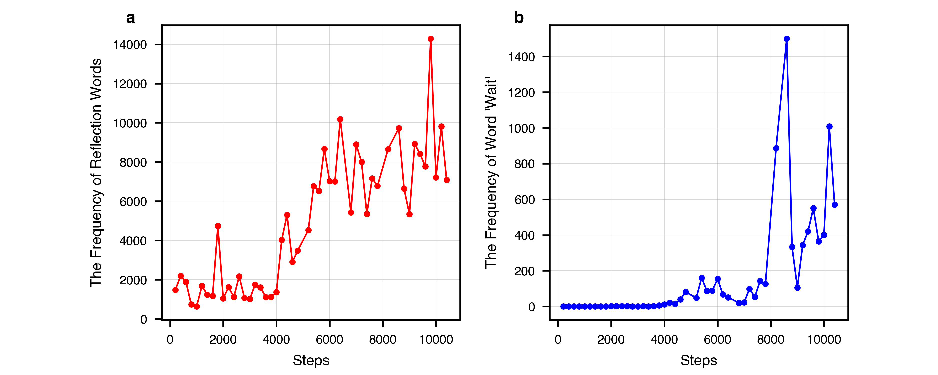
\includegraphics[width=\linewidth]{../papers/translations/r1-nature/assets/edfig1.pdf}
\end{center}
\phantomsection
\noindent\textbf{扩展数据图 1. 模型输出中与推理有关的语言特征随训练步数的演变.}\paperlabel{扩展数据 1}{r1n-edfig1}
a, 整个训练过程模型生成输出中具有代表性的反思词语的频数. 这些反思词语包括 wait (等等)、mistake (错误)、however (然而)、but (但是)、retry (重试)、error (错误)、verify (验证)、wrong (错了)、evaluate (评估) 和 check (检查). 这些词由三位人类专家组成的小组识别和整理. 每位专家独立提出一组能表示反思式推理的词, 随后通过共识合并为最终词表. b, 训练期间模型输出中单词 wait 的频数. 该词在训练初期几乎不存在, 在 4,000--7,000 步间零星出现, 在 8,000 步后频数显著增加. 这些趋势表明, 随训练推进, 时间推理或自我监控行为可能涌现.

\noindent\textbf{图中文字对应.} The Frequency of Reflection Words: 反思词语的频数; The Frequency of Word ``Wait'': 单词 wait 的频数; Steps: 训练步数. a、b 面板及原始曲线、坐标刻度全部保留.

\begin{center}
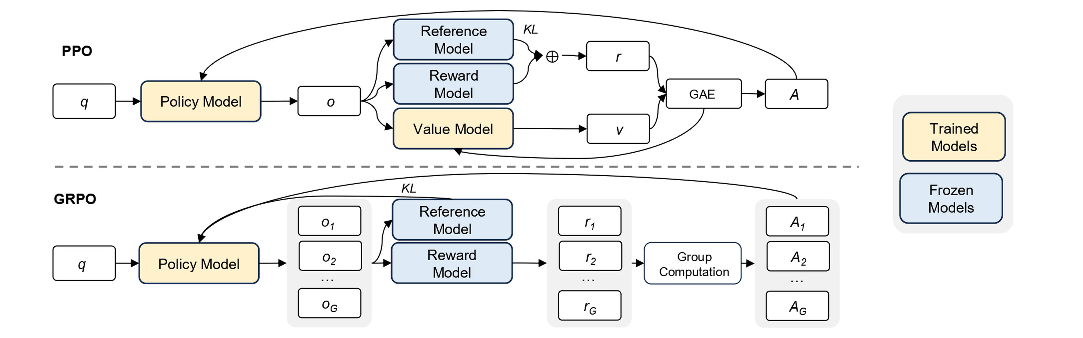
\includegraphics[width=\linewidth]{../papers/translations/r1-nature/assets/edfig2.pdf}
\end{center}
\phantomsection
\noindent\textbf{扩展数据图 2. 所提出的、用于基于 RL 训练的 GRPO 示意图.}\paperlabel{扩展数据 2}{r1n-edfig2}
在所提框架中, LLM 作为策略模型, 在给定查询 $q$ 的条件下生成回复 $\{o_1,o_2,\ldots,o_G\}$. 组内每条回复由奖励模型评估: 奖励模型可以是学习得到的 (基于模型), 也可以是人工指定的 (基于规则), 从而分配一个标量奖励信号. 随后, GRPO 按各组成员获得的奖励计算其相对优势. 与 PPO 不同, GRPO 不依赖显式价值函数, 而是直接从组内奖励分布估计优势. 随后更新策略参数, 最大化期望奖励, 同时尽量减少相对参考策略的偏离, 这种偏离通常用 KL 散度量化. 消除单独价值网络的需求, 使 GRPO 成为 PPO 等传统行动者--评论家方法的一种简化且有效的替代方案.

\noindent\textbf{图中文字对应.} Policy Model: 策略模型; Reference Model: 参考模型; Reward Model: 奖励模型; Value Model: 价值模型; Group Computation: 组内计算; Trained Models: 训练的模型; Frozen Models: 冻结的模型. PPO、GRPO、KL、$q,o,o_i,r,r_i,v,A,A_i$ 与图中的运算、箭头按原样保留. GAE 为原图缩写, 指广义优势估计 (中文说明为译注).

\phantomsection
\noindent\textbf{扩展数据表 1. AIME 数据集的说明性示例.}\paperlabel{扩展数据 1}{r1n-edtable1}

\noindent\textbf{提示.} 设 $b\ge2$ 为整数. 若正整数 $n$ 在 $b$ 进制下恰有两位, 且两位数字之和为 $\sqrt n$, 则称 $n$ 为 $b$-beautiful (在 $b$ 进制下“美丽”). 例如, 81 在 13 进制下是美丽的, 因为 $81=\underline{6}\,\underline{3}_{13}$ 且 $6+3=\sqrt{81}$. 求使 $b$ 进制下美丽整数超过十个的最小整数 $b\ge2$. 请一步一步推理, 并将最后答案放在 \texttt{\textbackslash boxed\{\}} 中.

\noindent\textbf{评估.} 解析 \texttt{\textbackslash boxed\{\}} 中的最终答案, 使用基于规则的评分器判断它是否等于标准答案. 按需要对数值取舍入值, 并用 SymPy 解析表达式.

\noindent\textbf{原表注.} 展示的问题来自 2024 年 AIME. 模型的任务是解决该问题并按要求格式 (例如 ANSWER) 输出答案. 评估使用基于规则的评分系统判断正确性. 当且仅当模型输出与标准解完全一致时, 判为正确.

\originalsection{致谢、作者信息与出版声明}\label{r1n-author-info}
\noindent\textbf{致谢.} 本研究由 DeepSeek-AI 支持.

\noindent\textbf{作者现地址说明.} Fuli Luo: 中国北京, 独立研究者. Jinhao Tu: 中国上海, 建平中学. Kai Hu: 中国合肥, 中国科学技术大学. Kexin Huang、Wenqin Yu、Xinyuan Li、Yue Gong 与 Yujia He: 中国北京, 北京大学. Zijun Liu: 中国北京, 清华大学. Ziyang Song: 中国香港特别行政区, Citadel Securities.

\noindent\textbf{作者及所属机构.} 全部作者所属机构为中国杭州 DeepSeek-AI 团队. 完整姓名按正式原文顺序列在下一部分; 上述现地址说明同样按原文保留.

\noindent\textbf{作者贡献.} 所有作者都对本次发表作出贡献, 分别参与数据收集和整理、实验设计以及 LLM 训练框架搭建. 作者也参与实验设置的实现和测试、RL 流程改进以及结果分析. 所有贡献者讨论并认可科学发现. 本文由合作团队指定的一部分作者撰写, 并经过内部集体审阅. 所有作者均审阅并认可了稿件最终版本. 核心贡献者为 D.G.、D.Y.、H.Z.、J.S.、R.Z.、R.X.、Q.Z.、S.M.、P.W.、X.B.、X.Z.、X.Y.、Y.W.、Z.F.W.、Z.G.、Z.S.、Z.L.、Z.G. 这些被指定为核心贡献者的作者对工作作出同等贡献, 并按字母顺序列出. 其余作者同样对研究作出了重要贡献, 姓名亦按字母顺序列出.

\noindent\textbf{通讯作者.} Wenfeng Liang, \texttt{wenfeng.liang@deepseek.com}.

\noindent\textbf{利益冲突.} 作者声明没有利益冲突, 并且不会就本稿内容申请专利.

\noindent\textbf{同行评审信息.} Nature 感谢 Edward Beeching、Yarin Gal、José Hernández-Orallo、Daphne Ippolito、Subbarao Kambhampati、Lewis Tunstall、Yiming Zhang 和 Lexin Zhou 对本工作同行评审的贡献. 同行评审报告可从原文章页面获取.

\noindent\textbf{出版者声明.} Springer Nature 对已发表地图中的管辖权主张及机构所属关系保持中立.

\noindent\textbf{补充信息条目.} 原文章另附 Supplementary Information, 含补充章节 1--11、补充表 1--29、补充图 1--16, 详见其目录; 另附 Peer Review file. 这两个独立文件未在本译文中镜像或全文翻译, 读者可从 \url{https://www.nature.com/articles/s41586-025-09422-z#MOESM1} 的文章页面相关条目访问.

\noindent\textbf{权利与许可.} 本文为开放获取, 按 Creative Commons Attribution 4.0 International License 许可发布. 该许可允许以任何媒介和格式使用、分享、改编、分发和复制, 条件是适当署名原作者与来源、提供许可链接并说明是否作出修改. 本文中的图像或其他第三方材料纳入文章的 Creative Commons 许可, 除非该材料的署名说明另有声明. 如果某材料未纳入文章许可, 且预期使用不受法律许可或超过法律允许范围, 则须直接向著作权人取得许可. 许可副本见 \url{https://creativecommons.org/licenses/by/4.0/}.

\noindent\textbf{原作者版权声明.} \copyright{} The Author(s) 2025.

\noindent\textbf{文章信息.} 投稿日期: 2025 年 2 月 14 日. 接受日期: 2025 年 7 月 17 日. 发表日期与正式记录版本日期: 2025 年 9 月 17 日. 期刊期次日期: 2025 年 9 月 18 日. 正式引文为 Guo, D., Yang, D., Zhang, H. et al. \textit{DeepSeek-R1 incentivizes reasoning in LLMs through reinforcement learning}. \textit{Nature} 645, 633--638 (2025). \url{https://doi.org/10.1038/s41586-025-09422-z}.

\originalsection{完整作者署名}\label{r1n-authors}
Daya Guo, Dejian Yang, Haowei Zhang, Junxiao Song, Peiyi Wang, Qihao Zhu, Runxin Xu, Ruoyu Zhang, Shirong Ma, Xiao Bi, Xiaokang Zhang, Xingkai Yu, Yu Wu, Z. F. Wu, Zhibin Gou, Zhihong Shao, Zhuoshu Li, Ziyi Gao, Aixin Liu, Bing Xue, Bingxuan Wang, Bochao Wu, Bei Feng, Chengda Lu, Chenggang Zhao, Chengqi Deng, Chong Ruan, Damai Dai, Deli Chen, Dongjie Ji, Erhang Li, Fangyun Lin, Fucong Dai, Fuli Luo, Guangbo Hao, Guanting Chen, Guowei Li, H. Zhang, Hanwei Xu, Honghui Ding, Huazuo Gao, Hui Qu, Hui Li, Jianzhong Guo, Jiashi Li, Jingchang Chen, Jingyang Yuan, Jinhao Tu, Junjie Qiu, Junlong Li, J. L. Cai, Jiaqi Ni, Jian Liang, Jin Chen, Kai Dong, Kai Hu, Kaichao You, Kaige Gao, Kang Guan, Kexin Huang, Kuai Yu, Lean Wang, Lecong Zhang, Liang Zhao, Litong Wang, Liyue Zhang, Lei Xu, Leyi Xia, Mingchuan Zhang, Minghua Zhang, Minghui Tang, Mingxu Zhou, Meng Li, Miaojun Wang, Mingming Li, Ning Tian, Panpan Huang, Peng Zhang, Qiancheng Wang, Qinyu Chen, Qiushi Du, Ruiqi Ge, Ruisong Zhang, Ruizhe Pan, Runji Wang, R. J. Chen, R. L. Jin, Ruyi Chen, Shanghao Lu, Shangyan Zhou, Shanhuang Chen, Shengfeng Ye, Shiyu Wang, Shuiping Yu, Shunfeng Zhou, Shuting Pan, S. S. Li, Shuang Zhou, Shaoqing Wu, Tao Yun, Tian Pei, Tianyu Sun, T. Wang, Wangding Zeng, Wen Liu, Wenfeng Liang, Wenjun Gao, Wenqin Yu, Wentao Zhang, W. L. Xiao, Wei An, Xiaodong Liu, Xiaohan Wang, Xiaokang Chen, Xiaotao Nie, Xin Cheng, Xin Liu, Xin Xie, Xingchao Liu, Xinyu Yang, Xinyuan Li, Xuecheng Su, Xuheng Lin, X. Q. Li, Xiangyue Jin, Xiaojin Shen, Xiaosha Chen, Xiaowen Sun, Xiaoxiang Wang, Xinnan Song, Xinyi Zhou, Xianzu Wang, Xinxia Shan, Y. K. Li, Y. Q. Wang, Y. X. Wei, Yang Zhang, Yanhong Xu, Yao Li, Yao Zhao, Yaofeng Sun, Yaohui Wang, Yi Yu, Yichao Zhang, Yifan Shi, Yiliang Xiong, Ying He, Yishi Piao, Yisong Wang, Yixuan Tan, Yiyang Ma, Yiyuan Liu, Yongqiang Guo, Yuan Ou, Yuduan Wang, Yue Gong, Yuheng Zou, Yujia He, Yunfan Xiong, Yuxiang Luo, Yuxiang You, Yuxuan Liu, Yuyang Zhou, Y. X. Zhu, Yanping Huang, Yaohui Li, Yi Zheng, Yuchen Zhu, Yunxian Ma, Ying Tang, Yukun Zha, Yuting Yan, Z. Z. Ren, Zehui Ren, Zhangli Sha, Zhe Fu, Zhean Xu, Zhenda Xie, Zhengyan Zhang, Zhewen Hao, Zhicheng Ma, Zhigang Yan, Zhiyu Wu, Zihui Gu, Zijia Zhu, Zijun Liu, Zilin Li, Ziwei Xie, Ziyang Song, Zizheng Pan, Zhen Huang, Zhipeng Xu, Zhongyu Zhang, Zhen Zhang.

Wenqin Yu 的 ORCID: \url{https://orcid.org/0000-0002-5715-3011}.

\begin{thebibliography}{99}
\bibitem{r1n-ref1} Brown, T. B. et al. Language models are few-shot learners. In Advances in Neural Information Processing Systems 33 (eds Larochelle, H. et al.) (ACM, 2020). 题名中译: 语言模型是少样本学习器.
\bibitem{r1n-ref2} OpenAI et al. GPT4 technical report. Preprint at \url{https://doi.org/10.48550/arXiv.2303.08774} (2024). 题名中译: GPT4 技术报告.
\bibitem{r1n-ref3} Wei, J. et al. Chain-of-thought prompting elicits reasoning in large language models. In Advances in Neural Information Processing Systems 35 (eds Koyejo, S. et al.) 24824--24837 (ACM, 2022). 题名中译: 思维链提示激发大语言模型中的推理.
\bibitem{r1n-ref4} Wei, J. et al. Emergent abilities of large language models. In Transactions on Machine Learning Research (eds Kamath, G. et al.) (2022). 题名中译: 大语言模型的涌现能力.
\bibitem{r1n-ref5} Kaplan, J. et al. Scaling laws for neural language models. Preprint at \url{https://doi.org/10.48550/arXiv.2001.08361} (2020). 题名中译: 神经语言模型的缩放定律.
\bibitem{r1n-ref6} Kojima, T., Gu, S. S., Reid, M., Matsuo, Y. \& Iwasawa, Y. Large language models are zero-shot reasoners. In Advances in Neural Information Processing Systems 35 (eds Oh, A. H. et al.) 22199--22213 (ACM, 2022). 题名中译: 大语言模型是零样本推理者.
\bibitem{r1n-ref7} Chung, H. W. et al. Scaling instruction-finetuned language models. J. Mach. Learn. Res. 25, 1--53 (2024). 题名中译: 扩展经过指令微调的语言模型.
\bibitem{r1n-ref8} DeepSeek-AI et al. DeepSeek-V3 technical report. Preprint at \url{https://doi.org/10.48550/arXiv.2412.19437} (2025). 题名中译: DeepSeek-V3 技术报告.
\bibitem{r1n-ref9} Shao, Z. et al. DeepSeekMath: pushing the limits of mathematical reasoning in open language models. Preprint at \url{https://doi.org/10.48550/arXiv.2402.03300} (2024). 题名中译: DeepSeekMath: 推进开放语言模型数学推理的极限.
\bibitem{r1n-ref10} Wang, X. et al. Self-consistency improves chain of thought reasoning in language models. In 11th International Conference on Learning Representations (ICLR, 2023). 题名中译: 自一致性改进语言模型中的思维链推理.
\bibitem{r1n-ref11} Hendrycks, D. et al. Measuring massive multitask language understanding. In 9th International Conference on Learning Representations (ICLR, 2021). 题名中译: 衡量大规模多任务语言理解.
\bibitem{r1n-ref12} Gema, A. P. et al. Are we done with MMLU? In Proc. 2025 Conference of the Nations of the Americas Chapter of the Association for Computational Linguistics: Human Language Technologies (eds Chiruzzo, L. et al.) Vol. 1 (Long Papers), 5069--5096 (ACL, 2025). 题名中译: 我们已经完成 MMLU 的工作了吗?.
\bibitem{r1n-ref13} Wang, Y. et al. MMLU-Pro: a more robust and challenging multi-task language understanding benchmark. In Advances in Neural Information Processing Systems 37 (eds Globersons, A. et al.) 95266--95290 (ACM, 2024). 题名中译: MMLU-Pro: 更稳健、更具挑战性的多任务语言理解基准.
\bibitem{r1n-ref14} Dua, D. et al. DROP: a reading comprehension benchmark requiring discrete reasoning over paragraphs. In Proc. 2019 Conference of the North American Chapter of the Association for Computational Linguistics: Human Language Technologies Vol. 1 (Long and Short Papers) (eds Burstein, J. et al.) 2368--2378 (ACL, 2019). 题名中译: DROP: 需要对段落进行离散推理的阅读理解基准.
\bibitem{r1n-ref15} Huang, Y. et al. C-EVAL: a multi-level multi-discipline Chinese evaluation suite for foundation models. In Advances in Neural Information Processing Systems 36 (eds Oh, A. et al.) 62991--63010 (ACM, 2023). 题名中译: C-EVAL: 面向基础模型的多层次、多学科中文评估套件.
\bibitem{r1n-ref16} Zhou, J. et al. Instruction-following evaluation for large language models. Preprint at \url{https://doi.org/10.48550/arXiv.2311.07911} (2023). 题名中译: 大语言模型的指令遵循评估.
\bibitem{r1n-ref17} Krishna, S. et al. Fact, fetch, and reason: a unified evaluation of retrieval-augmented generation. In Proc. 2025 Conference of the Nations of the Americas Chapter of the Association for Computational Linguistics: Human Language Technologies Vol. 1 (Long Papers) 4745--4759 (ACL, 2025). 题名中译: 事实、获取与推理: 检索增强生成的统一评估.
\bibitem{r1n-ref18} Rein, D. et al. GPQA: a graduate-level Google-proof Q\&A benchmark. Preprint at \url{https://doi.org/10.48550/arXiv.2311.12022} (2023). 题名中译: GPQA: 研究生水平、无法轻易用 Google 检索作答的问答基准.
\bibitem{r1n-ref19} OpenAI. Introducing SimpleQA; \url{https://openai.com/index/introducing-simpleqa/} (2024). 题名中译: 介绍 SimpleQA.
\bibitem{r1n-ref20} He, Y. et al. Chinese SimpleQA: a Chinese factuality evaluation for large language models. In Proc. 63rd Annual Meeting of the Association for Computational Linguistics Vol. 1 (Long Papers), 19182--19208 (ACL, 2025). 题名中译: Chinese SimpleQA: 大语言模型的中文事实性评估.
\bibitem{r1n-ref21} Xu, L. et al. CLUE: a Chinese Language Understanding Evaluation benchmark. In Proc. 28th International Conference on Computational Linguistics (eds Scott, D. et al.) 4762--4772 (International Committee on Computational Linguistics, 2020). 题名中译: CLUE: 中文语言理解评估基准.
\bibitem{r1n-ref22} Dubois, Y., Galambosi, B., Liang, P. \& Hashimoto, T. B. Length-controlled AlpacaEval: a simple way to debias automatic evaluators. Preprint at \url{https://doi.org/10.48550/arXiv.2404.04475} (2025). 题名中译: 长度控制的 AlpacaEval: 消除自动评估器偏差的简单方法.
\bibitem{r1n-ref23} Li, T. et al. From crowdsourced data to high-quality benchmarks: Arena-Hard and BenchBuilder pipeline. Preprint at \url{https://doi.org/10.48550/arXiv.2406.11939} (2024). 题名中译: 从众包数据到高质量基准: Arena-Hard 与 BenchBuilder 流程.
\bibitem{r1n-ref24} OpenAI. Introducing SWE-bench verified; \url{https://openai.com/index/introducing-swe-bench-verified/} (2024). 题名中译: 介绍 SWE-bench Verified.
\bibitem{r1n-ref25} Aider. Aider LLM leaderboards; \url{https://aider.chat/docs/leaderboards/} (2024). 题名中译: Aider 大语言模型排行榜.
\bibitem{r1n-ref26} Jain, N. et al. LiveCodeBench: holistic and contamination free evaluation of large language models for code. In 13th International Conference on Learning Representations (ICLR, 2024). 题名中译: LiveCodeBench: 大语言模型代码能力的全面、无污染评估.
\bibitem{r1n-ref27} Mirzayanov, M. Codeforces; \url{https://codeforces.com/} (2025). 题名中译: Codeforces.
\bibitem{r1n-ref28} Chinese Mathematical Society (CMS). Chinese National High School Mathematics Olympiad; \url{https://www.cms.org.cn/Home/comp/comp/cid/12.html} (2024). 题名中译: 中国全国高中数学奥林匹克.
\bibitem{r1n-ref29} Mathematical Association of America. American Invitational Mathematics Examination; \url{https://maa.org/maa-invitational-competitions} (2024). 题名中译: 美国数学邀请赛.
\bibitem{r1n-ref30} OpenAI. Hello GPT-4o; \url{https://openai.com/index/hello-gpt-4o/} (2024). 题名中译: 你好, GPT-4o.
\bibitem{r1n-ref31} Schulman, J., Wolski, F., Dhariwal, P., Radford, A. \& Klimov, O. Proximal policy optimization algorithms. Preprint at \url{https://doi.org/10.48550/arXiv.1707.06347} (2017). 题名中译: 近端策略优化算法.
\bibitem{r1n-ref32} Ouyang, L. et al. Training language models to follow instructions with human feedback. In Advances in Neural Information Processing Systems 35 (eds Koyejo, S. et al.) 27730--27744 (ACM, 2022). 题名中译: 利用人类反馈训练遵循指令的语言模型.
\bibitem{r1n-ref33} Nano et al. deepseek-ai/DeepSeek-R1: v1.0.0. Zenodo \url{https://doi.org/10.5281/zenodo.15753192} (2025). 题名中译: deepseek-ai/DeepSeek-R1: v1.0.0.
\bibitem{r1n-ref34} Yu, X. et al. deepseek-ai/DeepSeek-V3: v1.0.0. Zenodo \url{https://doi.org/10.5281/zenodo.15753346} (2025). 题名中译: deepseek-ai/DeepSeek-V3: v1.0.0.
\bibitem{r1n-ref35} Paszke, A. et al. PyTorch: an imperative style, high-performance deep learning library. In Advances in Neural Information Processing Systems 32 (eds Wallach, H. M. et al.) 8026--8037 (ACM, 2019). 题名中译: PyTorch: 命令式、高性能的深度学习库.
\bibitem{r1n-ref36} Kwon, W. et al. Efficient memory management for large language model serving with PagedAttention. In Proc. ACM SIGOPS 29th Symposium on Operating Systems Principles 611--626 (ACM, 2023). 题名中译: 用 PagedAttention 高效管理大语言模型服务的内存.
\end{thebibliography}

\label{r1n-end}
